\chapwithtoc{Introduction}\label{chap:introduction}

\section*{Game engines}

Game engines are used to create video games, which makes it part of a very big industry. Video games need to do massive realtime calculations on consumer hardware, which often makes game engines showcase some of the most impressive algorithms and techniques, mainly related to computer graphics. Game engines exist in various types and flavours, like smaller ones that are made for academic research or to make lightweight games as simple and straight-forward as possible to implement. Other game engines are backed by big companies and are feature-rich, tailored towards performant implementation of big and graphically advanced games.

Game engines range from simple libraries that introduce often used functions for rendering, animation, sound and more to whole frameworks that manage the complete execution flow of the game. There are even big editor programs that build a game from scripts and configuration made in a graphical user interface, which often include graphical editors for scene layout, animations, shaders, asset file management and more.

\section*{Entity Component System}

\begin{figure}
\centering
\tikzstyle{box}=[rectangle,draw,rounded corners=0.5ex,minimum height=0.5cm,minimum width=1.5cm]
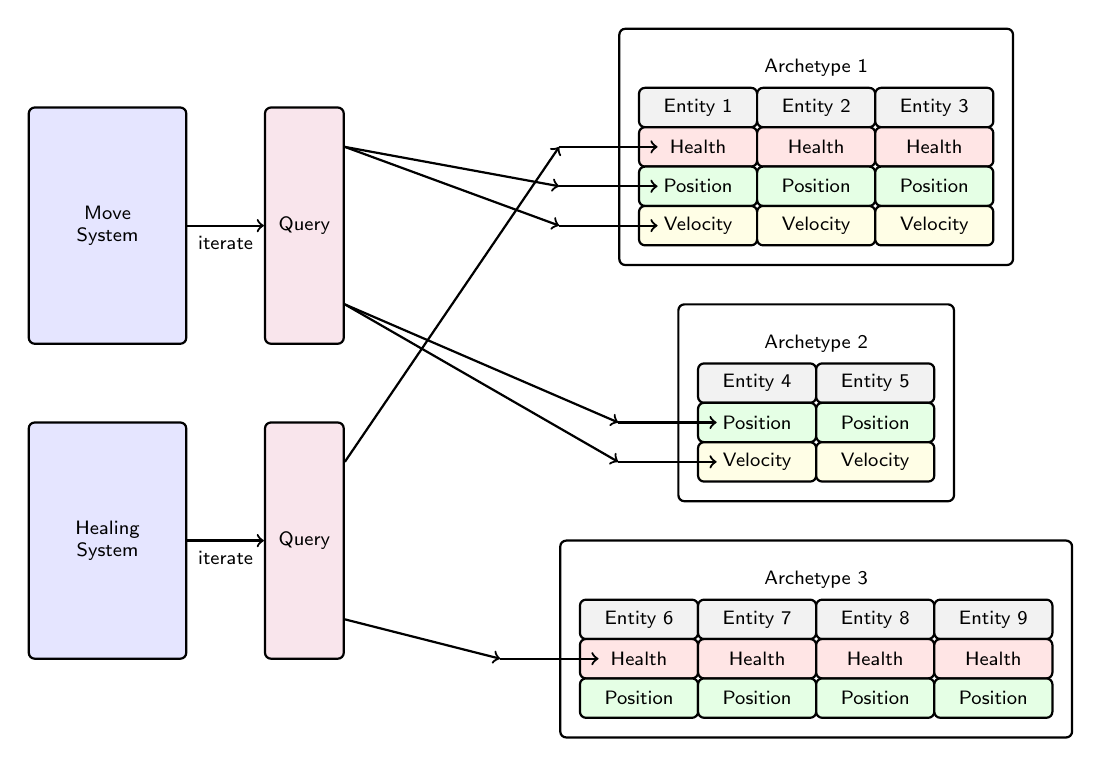
\begin{tikzpicture}[thick,font=\sf\scriptsize]
\node[box,minimum height=3cm,minimum width=5cm] at (0,0) {};
\node[] at (0,1) {Archetype 1};
\node[box,fill=gray!10] at (-1.5,0.5) {Entity 1};
\node[box,fill=gray!10] at (0,0.5) {Entity 2};
\node[box,fill=gray!10] at (1.5,0.5) {Entity 3};
\node[box,fill=red!10] (a1h) at (-1.5,0) {Health};
\node[box,fill=red!10] at (0,0) {Health};
\node[box,fill=red!10] at (1.5,0) {Health};
\node[box,fill=green!10] (a1p) at (-1.5,-0.5) {Position};
\node[box,fill=green!10] at (0,-0.5) {Position};
\node[box,fill=green!10] at (1.5,-0.5) {Position};
\node[box,fill=yellow!10] (a1v) at (-1.5,-1) {Velocity};
\node[box,fill=yellow!10] at (0,-1) {Velocity};
\node[box,fill=yellow!10] at (1.5,-1) {Velocity};

\node[box,minimum height=2.5cm,minimum width=3.5cm] at (0,-3.25) {};
\node[] at (0,-2.5) {Archetype 2};
\node[box,fill=gray!10] at (-0.75,-3) {Entity 4};
\node[box,fill=gray!10] at (0.75,-3) {Entity 5};
\node[box,fill=green!10] (a2p) at (-0.75,-3.5) {Position};
\node[box,fill=green!10] at (0.75,-3.5) {Position};
\node[box,fill=yellow!10] (a2v) at (-0.75,-4) {Velocity};
\node[box,fill=yellow!10] at (0.75,-4) {Velocity};

\node[box,minimum height=2.5cm,minimum width=6.5cm] at (0,-6.25) {};
\node[] at (0,-5.5) {Archetype 3};
\node[box,fill=gray!10] at (-2.25,-6) {Entity 6};
\node[box,fill=gray!10] at (-0.75,-6) {Entity 7};
\node[box,fill=gray!10] at (0.75,-6) {Entity 8};
\node[box,fill=gray!10] at (2.25,-6) {Entity 9};
\node[box,fill=red!10] (a3h) at (-2.25,-6.5) {Health};
\node[box,fill=red!10] at (-0.75,-6.5) {Health};
\node[box,fill=red!10] at (0.75,-6.5) {Health};
\node[box,fill=red!10] at (2.25,-6.5) {Health};
\node[box,fill=green!10] (a3p) at (-2.25,-7) {Position};
\node[box,fill=green!10] at (-0.75,-7) {Position};
\node[box,fill=green!10] at (0.75,-7) {Position};
\node[box,fill=green!10] at (2.25,-7) {Position};

\node[box,align=center,fill=blue!10,minimum height=3cm,minimum width=2cm] (gs) at (-9,-1) {Move\\System};
\node[box,align=center,fill=purple!10,minimum height=3cm,minimum width=1cm] (gsq) at (-6.5,-1) {Query};
\draw[->] (gs) -- node[midway,anchor=north] {iterate} (gsq);
\draw[->] ([yshift=1cm] gsq.east) -- ([xshift=-1cm] a1p.west);
\draw[->] ([xshift=-1cm] a1p.west) -- ([xshift=0.25cm] a1p.west);
\draw[->] ([yshift=1cm] gsq.east) -- ([xshift=-1cm] a1v.west);
\draw[->] ([xshift=-1cm] a1v.west) -- ([xshift=0.25cm] a1v.west);
\draw[->] ([yshift=-1cm] gsq.east) -- ([xshift=-1cm] a2p.west);
\draw[->] ([xshift=-1cm] a2p.west) -- ([xshift=0.25cm] a2p.west);
\draw[->] ([yshift=-1cm] gsq.east) -- ([xshift=-1cm] a2v.west);
\draw[->] ([xshift=-1cm] a2v.west) -- ([xshift=0.25cm] a2v.west);

\node[box,align=center,fill=blue!10,minimum height=3cm,minimum width=2cm] (ds) at (-9,-5) {Healing\\System};
\node[box,align=center,fill=purple!10,minimum height=3cm,minimum width=1cm] (dsq) at (-6.5,-5) {Query};
\draw[->] (ds) -- node[midway,anchor=north] {iterate} (dsq);
\draw[->] ([yshift=1cm] dsq.east) -- ([xshift=-1cm] a1h.west);
\draw[->] ([xshift=-1cm] a1h.west) -- ([xshift=0.25cm] a1h.west);
\draw[->] ([yshift=-1cm] dsq.east) -- ([xshift=-1cm] a3h.west);
\draw[->] ([xshift=-1cm] a3h.west) -- ([xshift=0.25cm] a3h.west);
\end{tikzpicture}
\caption{Example ECS structure (archetype based) with 3 archetypes and 2 systems. The \textit{Move System} queries and iterates over \textit{Position} and \textit{Velocity} components, the \textit{Healing System} over \textit{Health} components.}
\label{fig:ecs}
\end{figure}

The Entity Component System concept is not a single system, but rather an architectural pattern that is often used in game engines. It is based on the principle `composition over inheritance' and therefore uses a data-oriented design instead of an object oriented design. It models a \textit{world} in terms of components, entities and systems.

\textit{Components} are a single piece of data, like a simple struct, for example a player`s/NPC character`s \textit{Health} (Integer) or \textit{Velocity} (2D or 3D Vector). \textit{Entities} are usually just an identifier or index, that identifies a single collection of these (different) components that work together to create that entity implicitly. For single instance data, like \textit{Time} or \textit{Assets}, some ECSs introduce \textit{Resources} that can be used inside a system besides component queries to hold a single value that does not belong to any entity. Other ECSs use a \textit{Singleton entity} concept for that, which ensures that such a global resource is added to one entity only.

\textit{Systems} are functions that actually transform components from one state to the next, acting on a \textit{Query} of components, independent of the purpose of the corresponding entities. These systems should not hold any data themselves, as they are only meant to define the code that transforms a set of components. Systems can then be run by the engine in their order every frame for single threaded applications. For efficient multithreading, the systems can be scheduled in parallel while avoiding any race conditions or modification during iteration. This can be done by making sure only one system has write access to a specific component type at the same time.

Many ECS libraries are \textit{archetype} based. Archetypes group entities by the set of components types they have, meaning multiple entities usually belong to the same archetype, which all have the same components with potentially different values. In the example presented in \cref{fig:ecs}, \textit{Archetype 1} could represent player entities with a |Health|, |Position| and |Velocity| component, whereas \textit{Archetype 2} with |Position| and |Velocity| could represent any simple moving object, like bullets. \textit{Archetype 3} could represent stationary enemies with just a |Health| and |Position|. The \textit{Move System} iterates all entities with |Position| and |Velocity| to modifiy the entity`s position based on its velocity. The \textit{Healing System} just iterates over all |Health| components to increase the entity`s health over time.

\section*{Effekt language}

Effekt is a research programming language developed by the Software Engineering group at the Universität Tübingen. It has an effect system and features concepts like effects, effect handlers, bidirectional effects, compile-time polymorphism, existential types and complex control flow concepts using continuations and a `program stack'. The language has so far been used mostly for smaller algorithms and systems that use the features of the language to implement them much simpler than in other languages or to showcase its features.

\textit{Effects} are like generalized exceptions. An |effect| can be defined by a single operation (function) or an |interface| that defines multiple operations which need to be implemented to handle the effect. These operations can then be called anywhere in the program, which makes the used effect get statically added as part of the type of the surrounding function. This effect then needs to be handled by an \textit{effect handler} in the surrounding code, similar to an exception handler. Only programs (`main' functions) that do not have any unhandled effects left can be executed, which can be statically checked at compile time. When an effect operation gets called, execution jumps to the closest matching handler implementation of that effect, which takes the arguments defined in the effect operation signature. Inside the implementation, the code can jump back to the original callsite by calling `resume', which calls the continuation from before the effect operation was called. The `resume' call can also return a value to the original call site, as defined by the effect operation`s signature.

\section*{TODO (problem)}

TODO

\section*{Effekt game engine}

The main contribution of this thesis is the implementation of a simple 2D game engine using the Effekt language. That involved finding ways to use Effekt`s functionality as advantages in implement a game engine based on an ECS compared to existing approaches. As a side product, it also serves as a usability test and case study of the effekt language for a larger and more complicated project. To avoid implementing low-level window creation, graphics and input, the code is compiled to the \textsf{js-web} target for now. The `foreign function interface' (\textit{ffi}) is used to interoperate with javascript functions from Effekt code. On the web target, the browser allows us to use the javascript event loop for input events and the html5 \textsf{canvas} API for simple graphics using the \textit{ffi}.

A simple but fully functional ECS builds the basis for all other engine components. Features of the Effekt language are used to make very compact code with easily comprehensible logic, but very complex control flow. This leads to an implementation of the ECS in approximately 800 lines of code, which is quite short for its rich feature set. A html5 \textsf{canvas} 2D renderer and input system are built on top of the ECS, while also using the \textit{ffi}. Once the Effekt language and general ECS concepts are understood, usage of the engine is therefore straightforward.

\section*{Structure of the Thesis}

In this thesis we discuss some existing small or research-focused game engines and compare their working principles in chapter 1, introducing the Entity Component System architecture as well. In chapter 2 we go over the Effekt language and some of its most important features for this thesis. Then we describe the implementation of our game engine and its core differences to other game engines and ECSs in chapter 3. In chapter 4 we go over details of our game engine and how I used Effekt to make it easy to use. Then we present a case study of a `Snake' game implementation in chapter 5. Afterward, we discuss some improvements, limitations and possible future work in chapter 6. In the final chapter 7, we present our conclusion of the thesis.
